\chead{CHAPITRE 7. SPRINT 5 : Gestion des Congés et Tâches}

\chapter{Sprint 5: Gestion des Congés et Tâches}
\renewcommand{\mtctitle}{Sommaire}
\minitoc
\newpage
\section*{Introduction}
\addcontentsline{toc}{section}{\protect\numberline{}Introduction}%
Ce chapitre explore les étapes de la Sprint Gestion des Congés et Tâches, avec un accent particulier sur la gestion des demandes de congé et la supervision des tâches. Nous débuterons par un aperçu du backlog, avant de détailler la conception, la mise en œuvre et d’illustrer le travail effectué à l’aide de captures d’écran.

\section{Objectifs du Sprint}
L’objectif de cette sprint est de permettre la soumission et la validation des demandes de congé, la consultation et la gestion des tâches par les membres d’équipe, ainsi que la création de rapports de travail pour documenter l’avancement.

\section{Spécification des besoins}
\par Dans cette section, nous commencerons par présenter le diagramme des cas d’utilisation du sprint, puis nous exposerons le backlog associé.
\subsection{Diagramme cas d'utlisation du sprint 5}

\begin{figure}[H]
\centering
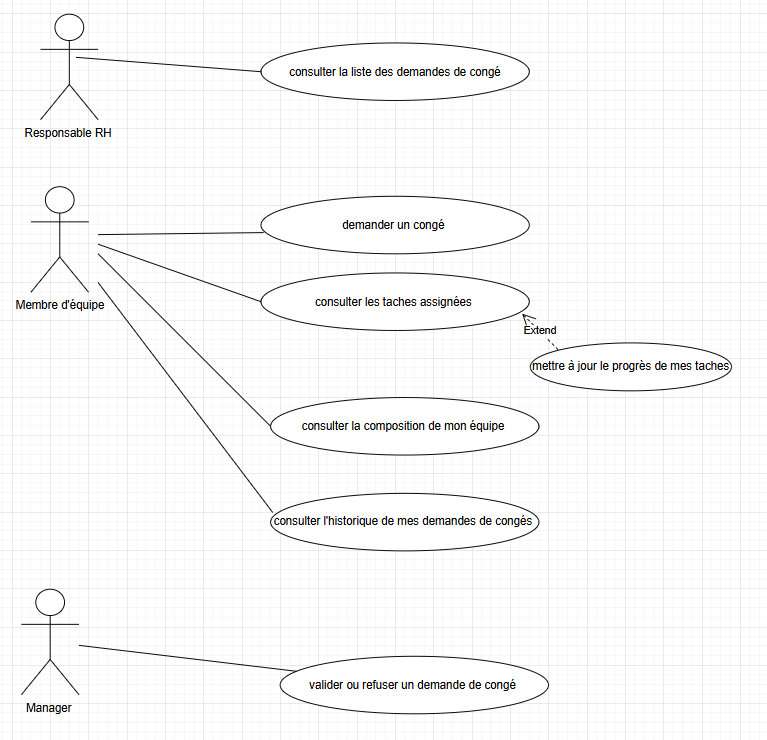
\includegraphics[width=15cm, height=12cm]{Figures/use case 5.png}
\caption{Diagramme de cas d’utilisation du Sprint 5}
\label{schema1}
\end{figure}

\subsection{ Sprint Backlog du sprint 5}
Le tableau ci-dessous présente le sprint backlog établi pour le cinquième sprint. Il récapitule les différentes user stories sélectionnées, accompagnées de leurs identifiants uniques, ainsi que les tâches techniques à réaliser pour chacune. Ce tableau permet d’avoir une vision claire et structurée du travail prévu, en facilitant la planification, la répartition des responsabilités et le suivi de l’avancement tout au long du sprint.
\begin{table}[H]
\caption{Backlog du sprint 5}
\centering
\begin{tabular}{|p{1cm}|p{8cm}|p{8cm}|}
\hline
\textbf{ID} & \textbf{User Story} & \textbf{Tâches techniques} \\
\hline
US-23 & En tant que membre d’équipe, je veux faire une demande de congé. 
& 
\begin{itemize}[leftmargin=*]
  \item Créer un formulaire de demande de congé.
  \item Valider les champs et enregistrer la demande.
  \item Sauvegarder la demande dans la base.
\end{itemize} \\
\hline
US-24 & En tant que manager, je veux valider ou refuser les demandes de congé des membres de mon équipe. 
& 
\begin{itemize}[leftmargin=*]
  \item Lister les demandes en attente.
  \item Ajouter les boutons d'approbation/refus.
  \item Mettre à jour le statut de la demande.
\end{itemize} \\
\hline
US-25 & En tant que responsable RH, je veux consulter la liste des demandes de congé. 
& 
\begin{itemize}[leftmargin=*]
  \item Concevoir l’interface d’affichage.
  \item Afficher toutes les demandes avec leurs statuts.
  \item Implémenter le tri et filtrage par statut.
\end{itemize} \\
\hline
US-26 & En tant que membre d’équipe, je veux consulter les tâches assignées. 
& 
\begin{itemize}[leftmargin=*]
  \item Créer une vue "mes tâches".
  \item Lier les tâches à l'utilisateur connecté.
  \item Afficher les tâches par priorité ou date.
\end{itemize} \\
\hline
US-27 & En tant que membre d’équipe, je veux consulter la composition de mon équipe. 
& 
\begin{itemize}[leftmargin=*]
  \item Ajouter une relation membre-équipe.
  \item Développer une interface de visualisation.
  \item Afficher la liste des membres de l’équipe.
\end{itemize} \\
\hline
US-28 & En tant que membre d’équipe, je veux mettre à jour le progrès de mes tâches. 
& 
\begin{itemize}[leftmargin=*]
  \item Ajouter un champ de progression dans chaque tâche.
  \item Enregistrer les modifications dans la base.
\end{itemize} \\
\hline
US-29 & En tant que membre d’équipe, je veux consulter l’historique de mes demandes de congés. 
& 
\begin{itemize}[leftmargin=*]
  \item Lister toutes les demandes de l'utilisateur.
  \item Ajouter une section historique avec filtre.
  \item Afficher les statuts de chaque demande.
\end{itemize} \\
\hline
\end{tabular}
\label{tab:sprint5_backlog}
\end{table}


\section{Analyse des besoins}
Avant de modéliser les fonctionnalités du système, il est essentiel de comprendre les besoins fonctionnels exprimés à travers les différents cas d’usage. La section suivante propose une description textuelle de ces cas d’utilisation, permettant de mieux cerner les interactions entre les utilisateurs et le système, et de poser les bases d’une modélisation cohérente.
    
\subsection{description textuelle de cas d'utilisation}

     \item \textbf{Cas d'utilisation "Valider ou refuser une demande de congé": } La table 7.2 ci-dessous présente la description textuelle du cas d'utilisation « Valider ou refuser une demande de congé ».

 \begin{table}[H]
 \caption{ Description textuelle du cas d’utilisation "Valider ou refuser une demande de congé"}
    \centering
    \begin{tabular}{|c|p{12cm}|}
    \hline
    \textbf{Titre} & Valider ou refuser une demande de congé \\
    \hline
    \textbf{Objectif} & Permettre au manager d’accepter ou refuser une demande de congé d’un membre d’équipe. \\
    \hline
    \textbf{Acteur}& Manager\\
    \hline
    \textbf{Pré-condition} & Une demande de congé doit avoir été soumise par un membre d’équipe et le manager doit être authentifié.
    \\
    \hline
    \textbf{Post-condition} & La décision (acceptation ou refus) est enregistrée et notifiée au membre d’équipe.\\
    \hline
    \textbf{Scénario nominal} & 1. Le manager accède à la liste des demandes de congé. \newline
    2. Il sélectionne une demande.\newline
    3. Il choisit d’accepter ou de refuser la demande.
    \newline
    4. Le système enregistre la décision.\\
    \hline
    \end{tabular}
    \label{tab:user_stories}
\end{table}


     \item \textbf{Cas d'utilisation "Demander un congé": } La table 7.3 ci-dessous présente la description textuelle du cas d'utilisation « Demander un congé ».

 \begin{table}[H]
 \caption{ Description textuelle du cas d’utilisation "Demander un congé"}
    \centering
    \begin{tabular}{|c|p{12cm}|}
    \hline
    \textbf{Titre} & Demander un congé \\
    \hline
    \textbf{Objectif} & Permettre au membre d’équipe de soumettre une demande de congé à son manager. \\
    \hline
    \textbf{Acteur}& Membre d’équipe\\
    \hline
    \textbf{Pré-condition} & Le membre d’équipe doit être authentifié et avoir un manager assigné.\\
    \hline
    \textbf{Post-condition} & La demande de congé est soumise et en attente de validation par le manager.\\
    \hline
    \textbf{Scénario nominal} & 1. Le membre d’équipe accède à l’interface de gestion des congés. \newline
    2. Il entre les détails de la demande (dates, motif).\newline
    3. Il soumet la demande au manager.
    \newline
    4. Le système enregistre la demande en attente de validation.
    \\
    \hline
    \end{tabular}
    \label{tab:user_stories}
\end{table}

     \item \textbf{Cas d'utilisation "Consulter les tâches": } La table 7.4 ci-dessous présente la description textuelle du cas d'utilisation « Consulter les tâches ».

 \begin{table}[H]
 \caption{ Description textuelle du cas d’utilisation "Consulter les tâches"}
    \centering
    \begin{tabular}{|c|p{12cm}|}
    \hline
    \textbf{Titre} & Consulter les tâches \\
    \hline
    \textbf{Objectif} & Permettre au membre d’équipe de visualiser les tâches assignées par le manager. \\
    \hline
    \textbf{Acteur}& Membre d’équipe\\
    \hline
    \textbf{Pré-condition} & Le membre d’équipe doit être authentifié et des tâches doivent lui être assignées par le manager.
    \\
    \hline
    \textbf{Post-condition} & La liste des tâches assignées est affichée avec leurs statuts.\\
    \hline
    \textbf{Scénario nominal} & 1. Le membre d’équipe accède à l’interface de gestion des tâches. \newline
    2. Il sélectionne l’option de consultation.\newline
    3. Le système affiche les tâches assignées par le manager.\newline
    4. Il consulte les détails.\\
    \hline
    \end{tabular}
    \label{tab:user_stories}
\end{table}


   

   

\section{Conception}
\hspace{0.5cm}\textbf Dans cette section, nous discutons de la conception du quatrième sprint. nous Commençons par le diagramme de classes du sprint. Ensuite, nous examinons la modélisation de quelques diagrammes de séquences . 

\subsection{Diagrammes de séquences}
Dans le cadre de l’analyse dynamique du système, un diagramme de séquence a été réalisé pour chaque fonctionnalité clé développée lors des sprints. Le diagramme ci-dessous illustre spécifiquement le scénario du cas d'utilisation « Demander un congé », permettant de visualiser les interactions entre le membre d'équipe et le système lors de la création d’un nouvel demande de congé.

\subsubsection{Diagramme de séquence au cas d’utilisation «Demander un congé»}

Cette figure illustre le déroulement du scénario associé à ce cas d'utilisation.
     \begin{figure}[H]
    \centering
    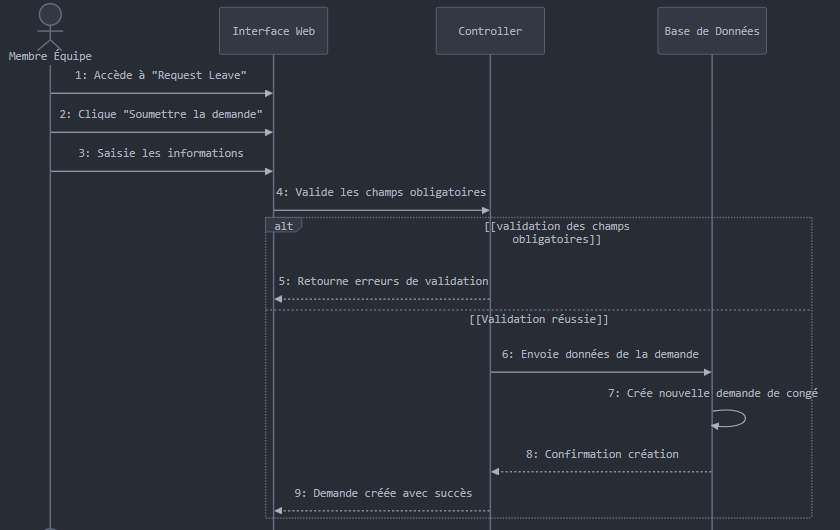
\includegraphics[width=18cm, height=23cm]{Figures/seq5.png}
    \caption{Diagramme de séquence au scénario «Demander un congé»}

\end{figure}

\section{Réalisation: Interfaces Utilisateur dans RhNova}
Dans cette dernière phase du projet, plusieurs interfaces ont été conçues pour faciliter la gestion des congés et des tâches au sein des équipes. Ces interfaces permettent aux utilisateurs de soumettre et suivre leurs demandes de congé, de gérer leurs tâches quotidiennes, et de consulter les informations relatives à leur équipe et à l’historique des congés.

\vspace{5mm}
\begin{itemize}
     \begin{itemize}
      \item \textbf{Suivre demandes de congé: }Cette interface permet au responsable RH de consulter la liste des demandes de congé soumises par les membres de l’équipe ainsi que leur état (approuvée, refusée ou en attente), afin d’assurer le suivi et la gestion administrative des absences.

      \end{itemize}
         \begin{figure}[H]
             \centering
             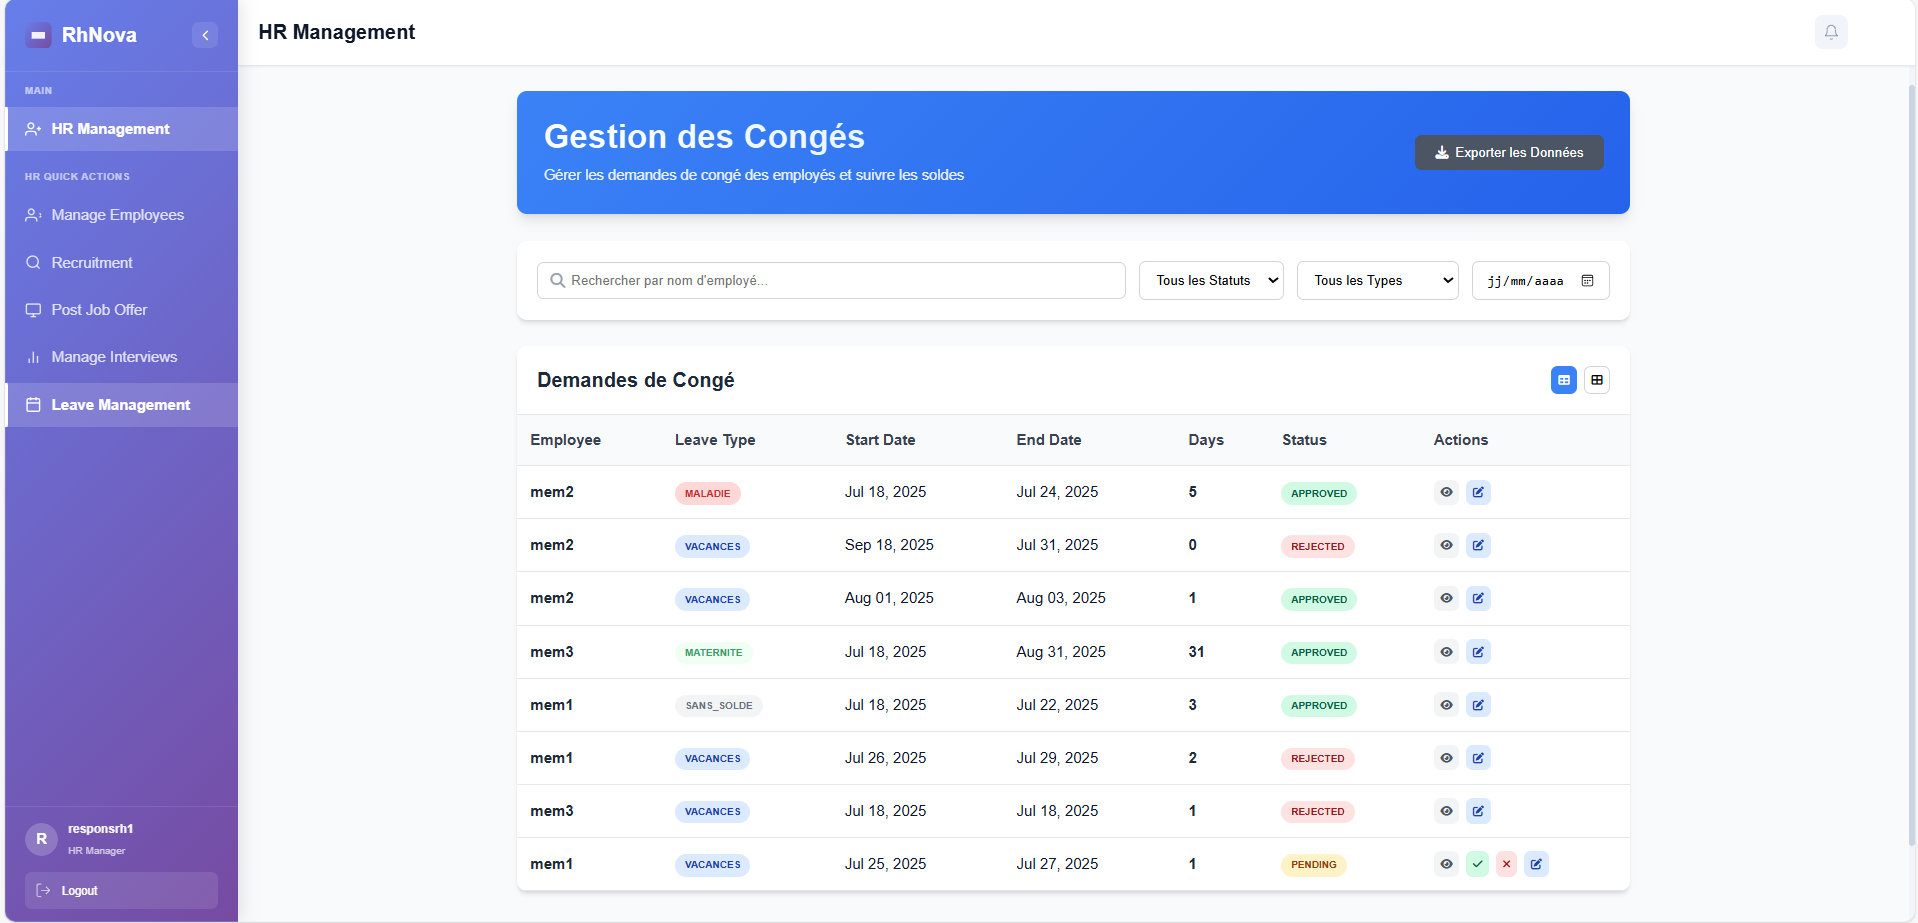
\includegraphics[width=\textwidth]{Figures/responscongé.png}
             \caption{Page de suivi des demandes congé}
         \end{figure}
              \end{itemize}
\begin{itemize}
         \item \textbf{Demande d'un congé : } Cette interface permet à un membre de l’équipe de soumettre une demande de congé en remplissant un formulaire avec le type de congé, la priorité, les dates de début et de fin, le motif et des notes éventuelles pour le manager. Elle facilite ainsi la communication et la gestion des absences au sein de l’organisation.
         
                  \begin{figure}[H]
             \centering
             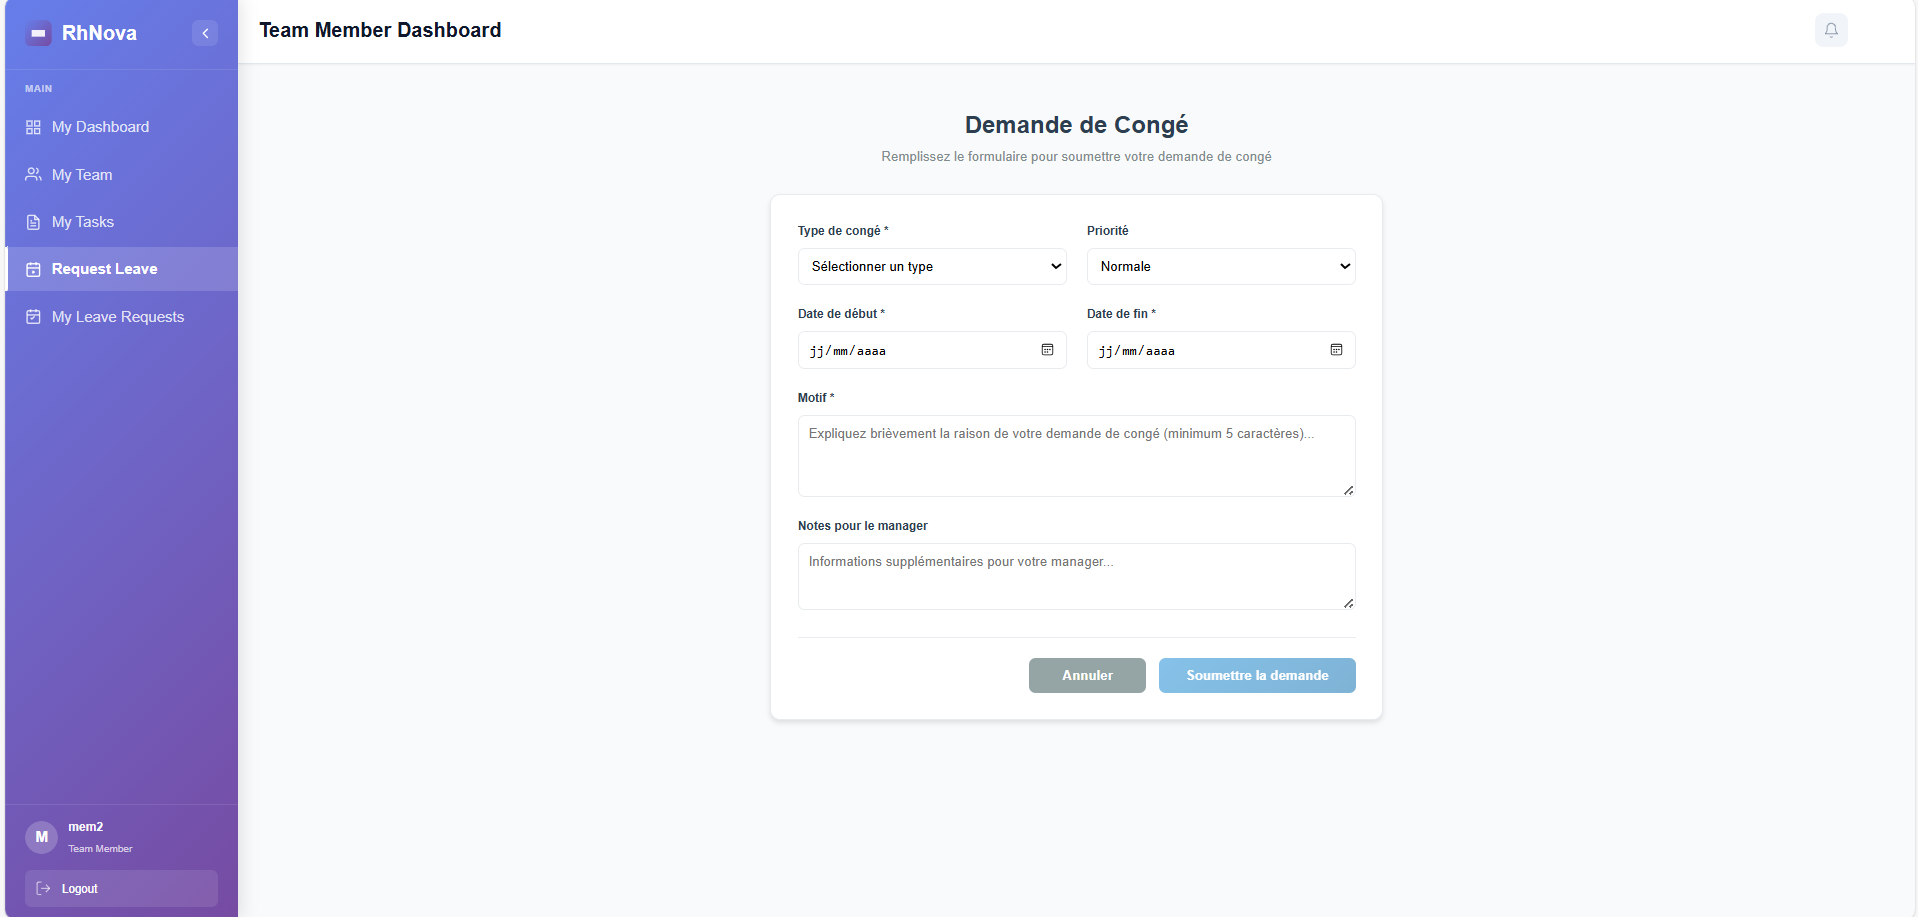
\includegraphics[width=\textwidth]{Figures/memdemande.png}
             \caption{Interface de demande de congé }
         \end{figure}
     \end{itemize}
     
\begin{itemize}
     \item\textbf{ Gestion des tâches  : }
Cette interface permet au membre d’équipe de consulter la liste des tâches qui lui ont été assignées par le manager, ainsi que leur état d’avancement et leur priorité. L’utilisateur peut également mettre à jour le pourcentage de progression ou changer le statut des tâches (en attente, en cours, terminée) afin d’assurer un meilleur suivi de son travail.
         \begin{figure}[H]
             \centering
             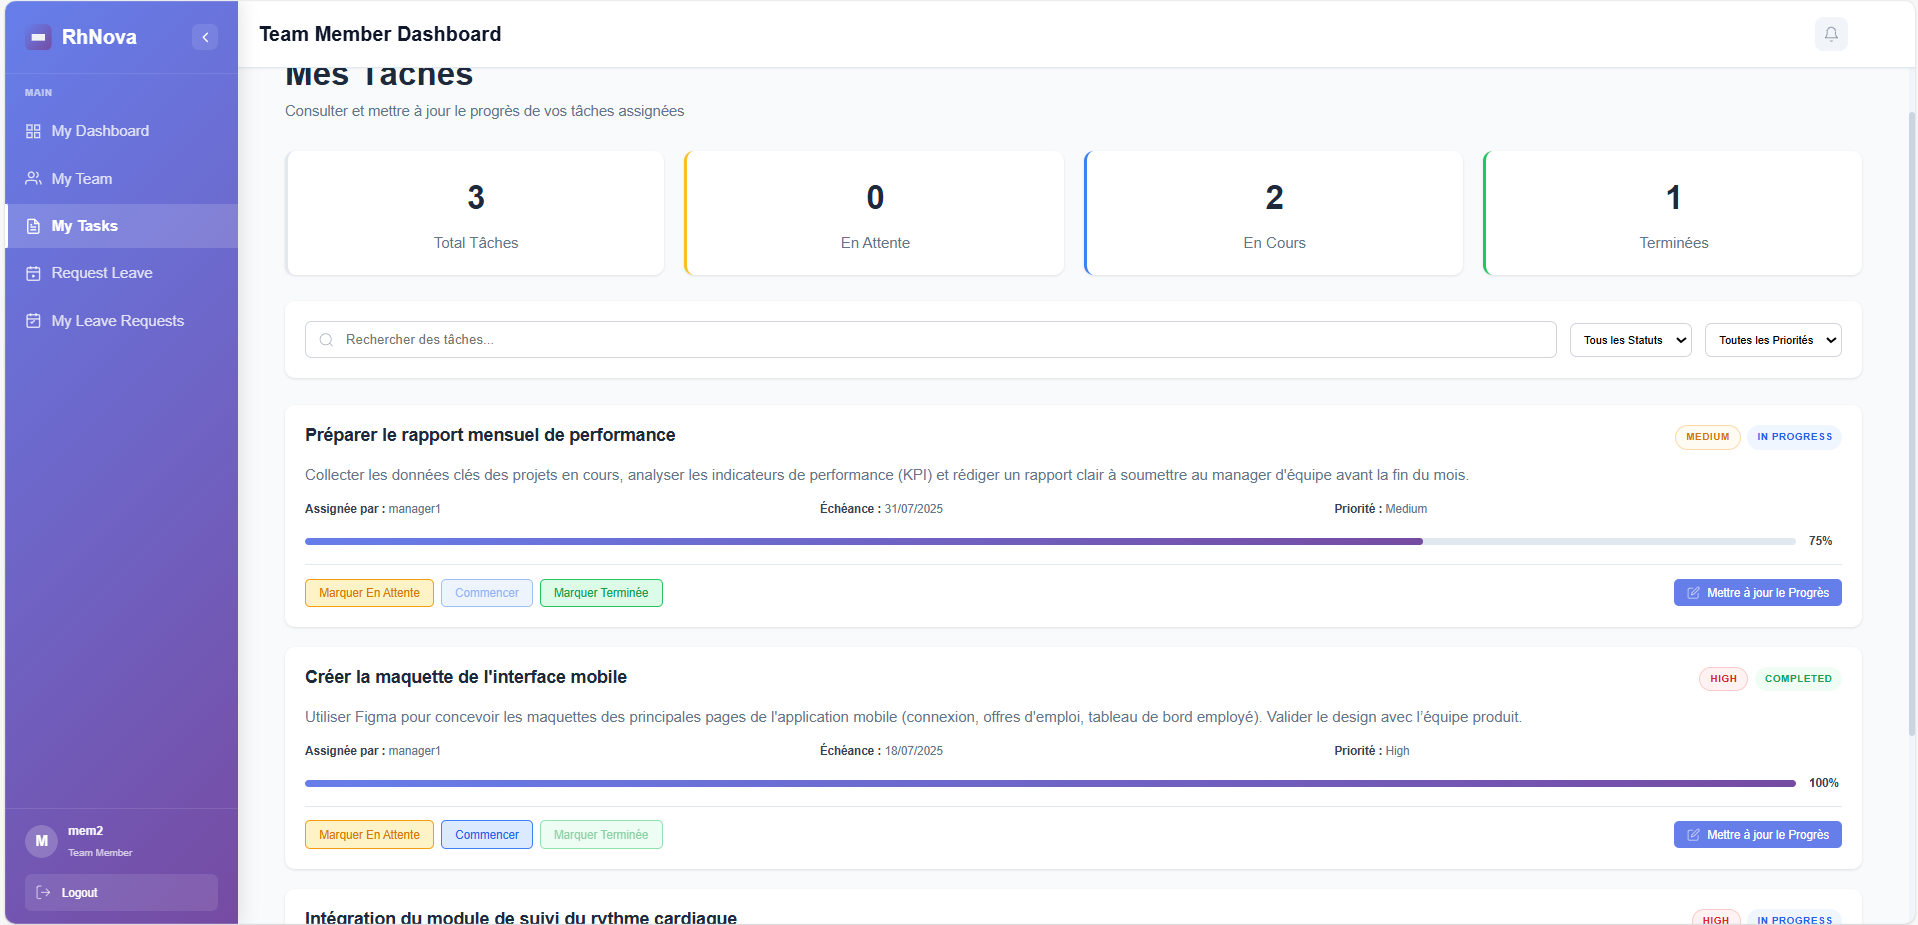
\includegraphics[width=\textwidth]{Figures/memtache.png}
             \caption{Interface de gestion des tâches }
         \end{figure}
     \end{itemize}
     
\begin{itemize}
     \item\textbf{  Consultation équipe   : }
Cette interface permet au membre d’équipe de visualiser les informations sur son équipe actuelle. Il peut voir le nom de l’équipe, son manager, la date de création, ainsi que la liste des membres avec leurs rôles et leurs adresses e-mail.     
         \begin{figure}[H]
             \centering
             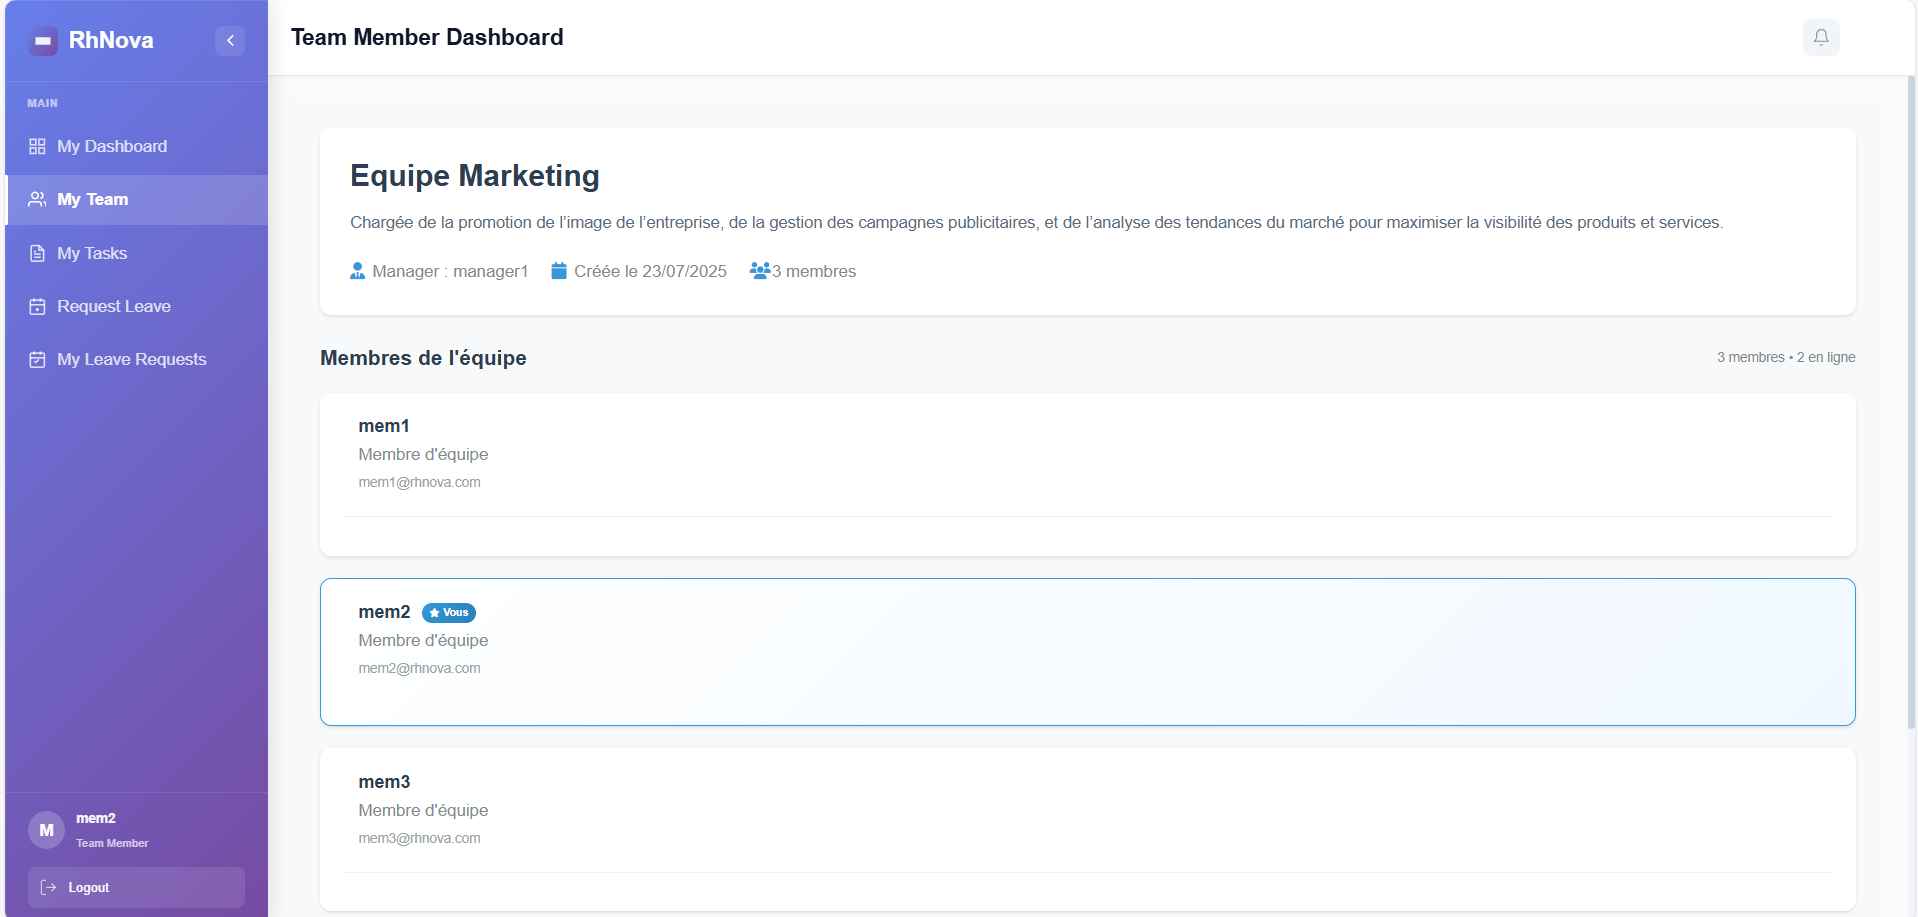
\includegraphics[width=\textwidth]{Figures/memequipe.png}
             \caption{Interface de consultation équipe }
         \end{figure}
     \end{itemize}
     
\begin{itemize}
     \item\textbf{  Consultation de l’historique des demandes de congé : }
Cette interface permet au membre d’équipe de visualiser l’historique complet de ses demandes de congé. Il peut voir le nombre de jours accordés, le statut de chaque demande (acceptée, refusée ou en attente), la période concernée, le type de congé, la raison, la date de soumission ainsi que les commentaires du manager.  
            \begin{figure}[H]
             \centering
             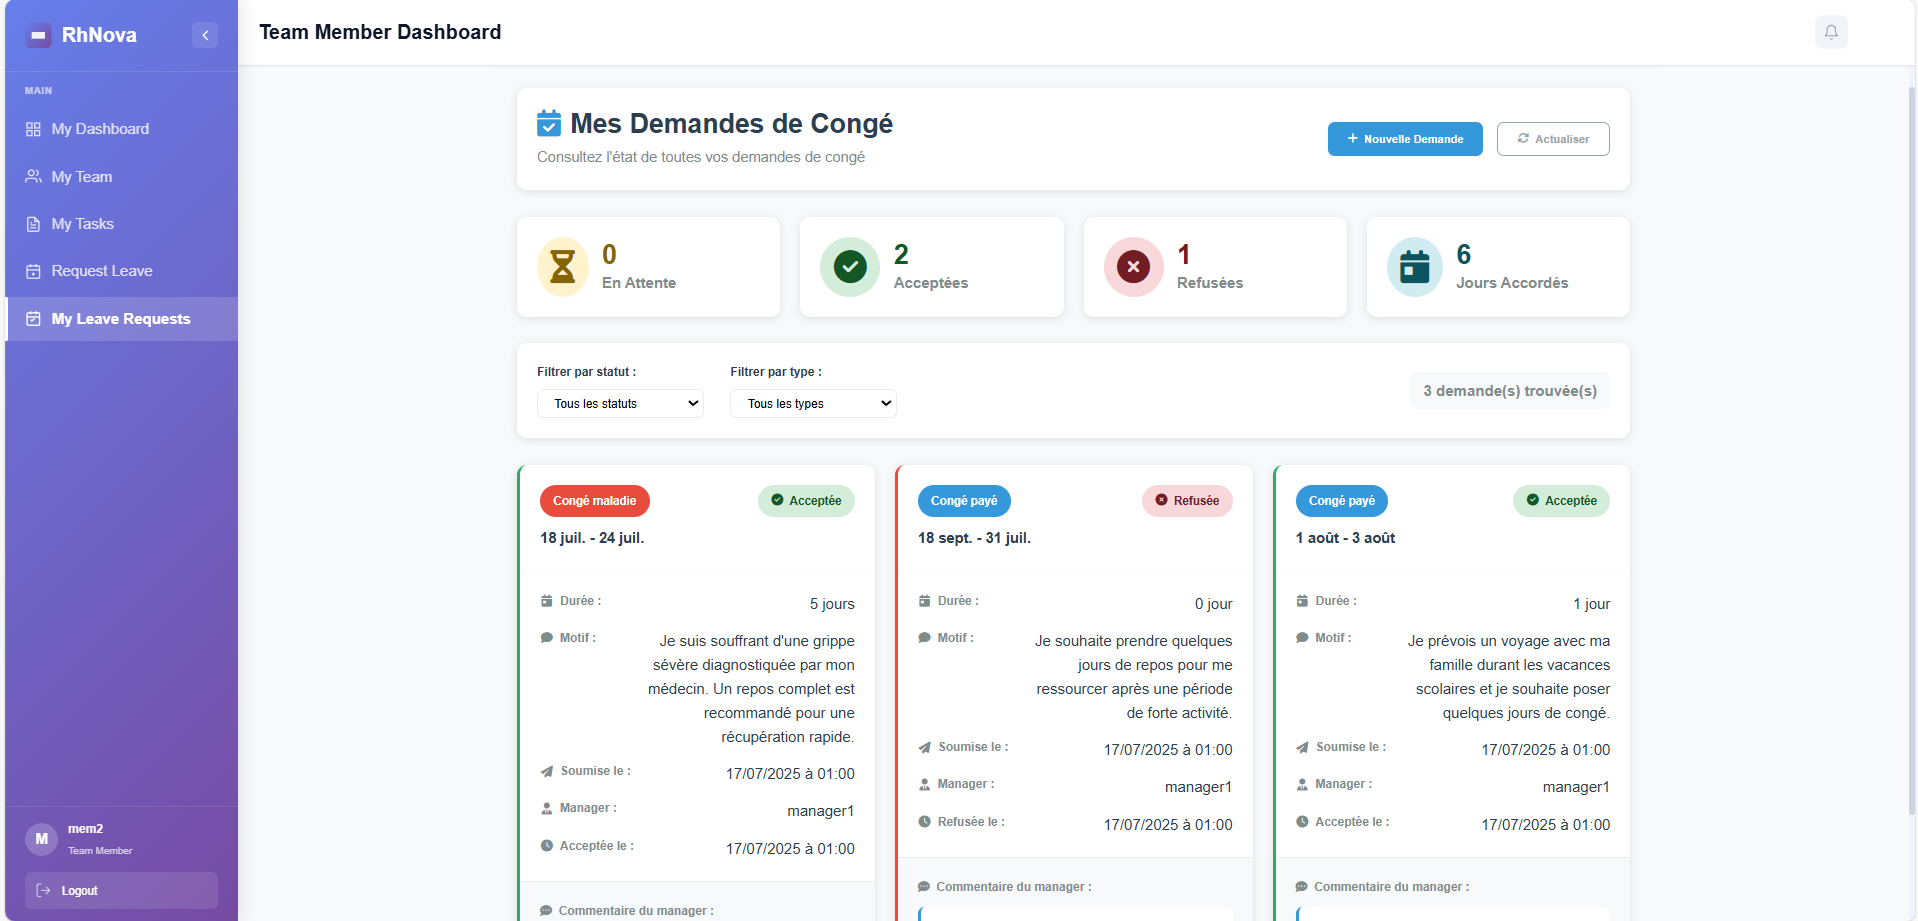
\includegraphics[width=\textwidth]{Figures/memhistorique.png}
             \caption{Interface de consultation de l’historique des demandes de congé}
         \end{figure}

     \end{itemize}
\begin{itemize}
         \item \textbf{Gestion des demandes de congé  : }Cette interface permet au manager de consulter et gérer toutes les demandes de congé soumises par les membres de son équipe. Il peut voir le détail de chaque demande (membre concerné, période, durée, motif, notes), identifier les demandes urgentes, et les approuver ou les refuser directement. 
         \begin{figure}[H]
             \centering
             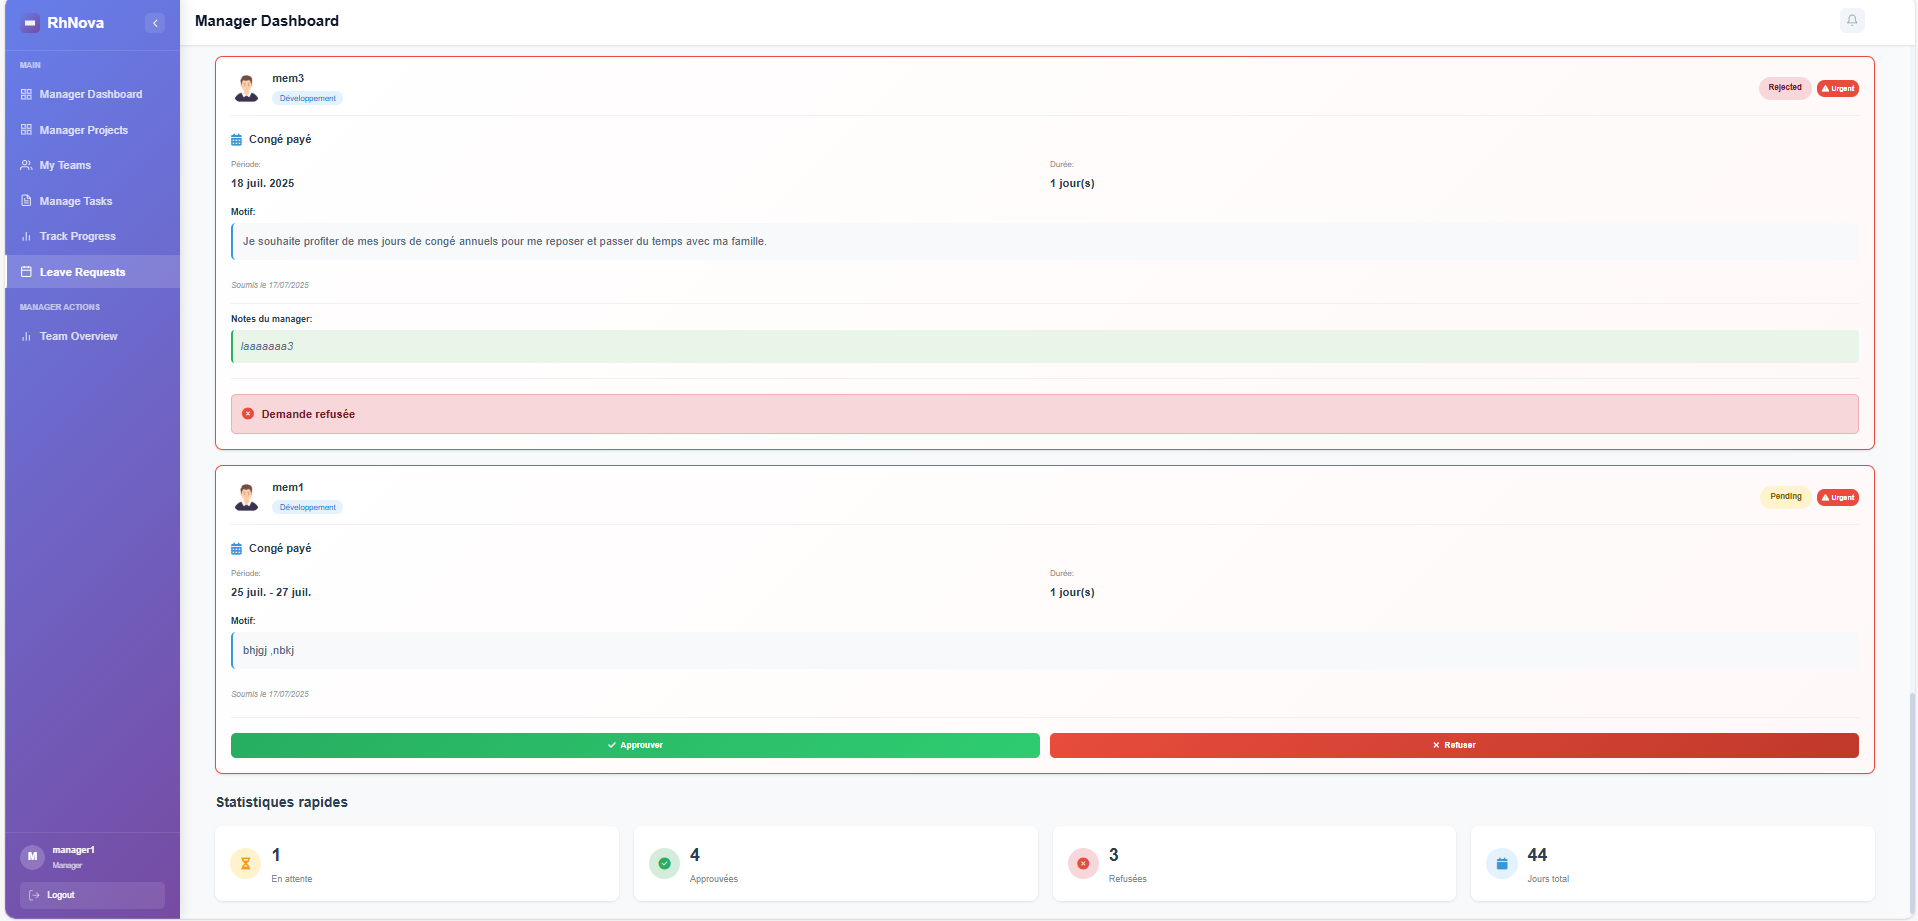
\includegraphics[width=\textwidth]{Figures/managercongé.png}
             \caption{Interface de gestion des demandes de congé }
         \end{figure}
     \end{itemize}


\section*{Conclusion}
En conclusion, ce chapitre a structuré la Sprint Gestion des Congés et Tâches, en définissant les objectifs et détaillant le backlog, tout en exposant les diagrammes de cas d’utilisation, classes et de séquences. Les descriptions textuelles et captures d’écran ont confirmé la mise en œuvre réussie, établissant un fondement solide pour la future gestion des ressources humaines.
\addcontentsline{toc}{section}{\protect\numberline{}Conclusion}%